\documentclass{amsart}
\usepackage{amsmath,amssymb,amsthm}
\usepackage{mathtools}
\usepackage[hidelinks]{hyperref}
\usepackage{graphicx}
\usepackage{enumitem}
\usepackage{algorithm}
\usepackage[noend]{algpseudocode}

% Theorem environments
\newtheorem{theorem}{Theorem}[section]
\newtheorem{lemma}[theorem]{Lemma}
\newtheorem{proposition}[theorem]{Proposition}
\newtheorem{corollary}[theorem]{Corollary}
\newtheorem{conjecture}[theorem]{Conjecture}

\theoremstyle{definition}
\newtheorem{definition}[theorem]{Definition}
\newtheorem{example}[theorem]{Example}

\theoremstyle{remark}
\newtheorem{remark}[theorem]{Remark}

\numberwithin{equation}{section}

% Import command files (if they exist)
\InputIfFileExists{commands/math}{}{}
\InputIfFileExists{commands/general}{}{}
\InputIfFileExists{commands/macros}{}{}

% Bibliography style
\bibliographystyle{amsplain}

\title[Phase Transitions in AI Alignment]{Phase Transitions in AI Alignment:
A Free Energy Principle Framework for Predicting Emergent Misalignment}

\author{NeuriCo}
\email{chicagohailab@gmail.com}

\date{June 26, 2026}

\subjclass[2020]{Primary 37G10, 37N25; Secondary 60H10, 94A17, 37M20}

\keywords{Cusp catastrophe, bifurcation, free energy principle, gradient flow,
critical transition, emergent misalignment, early-warning signals}

\begin{document}

\begin{abstract}
Empirical work in AI safety shows that finetuning a language model on a narrow malicious
task sometimes induces broad \emph{emergent misalignment} and sometimes does not, with no
predictive theory for when the failure occurs or how abrupt it is. We supply such a theory.
Modeling alignment as a variational free-energy gradient flow in the sense of the Free Energy
Principle, we derive---rather than posit---a scalar order parameter $m$ whose effective
potential is the cusp-catastrophe normal form
$F(m;a,h)=\tfrac14 b m^4+\tfrac12 a(\lambda)m^2-h(\lambda)m$, where $\lambda$ is the
intervention strength, $a(\lambda)$ an alignment stiffness, and $h(\lambda)$ a directional
bias. From this single two-parameter family we prove four results. First, a unique critical
threshold $\lambda^\ast$ separates robust alignment from misalignment, located exactly where
a Hessian eigenvalue crosses zero. Second, a symmetric ($h\equiv0$) intervention undergoes a
continuous supercritical pitchfork with mean-field exponent $\beta=\tfrac12$. Third, a biased
($h\neq0$) intervention unfolds the pitchfork into a fold, producing a discontinuous jump with
hysteresis on the cusp curve $27bh^2+4a^3=0$; this dichotomy unifies the two empirically
reported kinetic regimes. Fourth, near $\lambda^\ast$ the variance and autocorrelation time of
$m$ diverge, yielding a quantitative early-warning law. Proofs use Lyapunov--Schmidt and
center-manifold reduction, the gradient dynamic-transition theorem, and Ornstein--Uhlenbeck
analysis; every analytic claim is verified symbolically and numerically. Calibrated to reported
thresholds, the model classifies null versus emergent-misalignment outcomes with ROC-AUC
$0.996$ and threshold MAE $0.056$.

\end{abstract}

\maketitle

\section{Introduction}\label{sec:intro}

A central empirical puzzle in contemporary AI safety is \emph{emergent misalignment} (EM):
finetuning a large language model on a narrow, seemingly harmless dataset---insecure code,
or bad health advice---can cause the model to become broadly misaligned across unrelated
domains \cite{betley2025em,wang2025persona}. The phenomenon is fragile and regime-dependent.
The same intervention sometimes produces a null result (robust alignment), sometimes a gradual
drift, and sometimes a sudden behavioral collapse \cite{soligo2026em,nghiem2026trait}. There is,
at present, no predictive theory for \emph{when} an alignment intervention catastrophically
fails, nor for the \emph{order} of the failure (continuous versus abrupt), nor for early-warning
signals that precede it.

This is precisely the kind of question that the mathematics of \emph{critical transitions}
was built to answer. Bifurcation theory of fast--slow systems \cite{kuehn2011}, dynamic
transition theory for gradient flows \cite{mawang2008}, and the variational Free Energy
Principle (FEP) of theoretical biology \cite{friston2021} together supply order parameters,
threshold criteria, normal forms, and divergence laws. Yet this machinery has never been
applied to alignment, and the empirical EM literature uses none of its language. The two
bodies of work have remained disjoint. The contribution of this paper is to build the missing
bridge and to prove the theorems it implies.

\paragraph{The problem.}
We ask whether alignment dynamics can be modeled as variational free-energy minimization in
which a narrow misalignment intervention of strength $\lambda$ induces a phase transition in
the energy landscape, such that: (i) a critical threshold $\lambda^\ast$ separates robust
alignment from EM; (ii) the order of the transition is predictable; and (iii) the framework
predicts which intervention regimes yield a null result versus a sudden collapse, together with
quantitative precursors. The empirical literature poses exactly this and leaves it open,
remarking that the transition order ``may itself depend on the intervention regime''
\cite{nghiem2026trait,soligo2026em}.

\paragraph{Our approach and results.}
We model the misalignment order parameter $m\in\R$ (identified empirically with a toxic-persona
latent, the dominant principal component of trait drift, or a moral-susceptibility score) as
the internal coordinate of an FEP gradient flow $\dot m=-\partial_m F$. We then \emph{derive}
the effective potential from a two-component generative mixture: a Taylor expansion of the
FEP free energy about the aligned state yields the cusp-catastrophe normal form
\begin{equation}\label{eq:cusp-intro}
   F(m;a,h)=\tfrac14 b\,m^4+\tfrac12 a(\lambda)\,m^2-h(\lambda)\,m,\qquad b>0,
\end{equation}
with $a(\lambda)=a_0-c\lambda$ an alignment stiffness eroded by the intervention and
$h(\lambda)$ a directional bias set by its asymmetry. From the single family
\eqref{eq:cusp-intro} we prove:

\begin{itemize}[leftmargin=*,itemsep=2pt,topsep=2pt]
  \item \textbf{A critical threshold (Theorem~\ref{thm:threshold}).} The aligned equilibrium
    $m=0$ is asymptotically stable if and only if $a(\lambda)>0$, and loses stability when the
    Hessian eigenvalue crosses zero at the unique $\lambda^\ast=a_0/c$. Below $\lambda^\ast$:
    robust alignment. Above: emergent misalignment.
  \item \textbf{Order set by symmetry (Theorems~\ref{thm:pitchfork}--\ref{thm:fold}).}
    A symmetric intervention ($h\equiv0$) gives a supercritical pitchfork---a \emph{continuous}
    transition with mean-field exponent $\beta=\tfrac12$ (the gradual-LoRA regime). A biased
    intervention ($h\neq0$) unfolds the pitchfork into a fold (saddle-node), giving a
    \emph{catastrophic jump with hysteresis} on the exact cusp curve $27bh^2+4a^3=0$ (the
    full-finetune regime). This unifies the two empirical kinetic regimes in one normal form.
  \item \textbf{Early-warning laws (Theorem~\ref{thm:earlywarning}).} Near $\lambda^\ast$ the
    stationary variance and autocorrelation time of $m$ diverge (critical slowing down),
    giving a pre-failure precursor in which the internal order parameter \emph{leads} the
    behavioral jump.
\end{itemize}

\paragraph{Proof techniques.}
The threshold is a linear-stability calculation; the order of the transition follows from
center-manifold/Lyapunov--Schmidt reduction together with the gradient dynamic-transition
sign criterion of Ma--Wang \cite{mawang2008} and the catastrophic-bifurcation classification
of Kuehn \cite{kuehn2011}; the cusp curve is obtained by eliminating $m$ between $F'$ and
$F''$ (a resultant computation); the early-warning laws come from linearizing the governing
stochastic differential equation to an Ornstein--Uhlenbeck process. Every analytic claim is
checked symbolically (the resultant is recovered exactly as $b^2(4a^3+27bh^2)$) and numerically
(variance divergence, hysteresis folds matching the analytic curve to within $1\%$, and a
stationary law matching the Boltzmann form to a Jensen--Shannon divergence of
$6\times10^{-4}$ nats). Calibrated to the reported empirical thresholds, the model produces a
universality data-collapse and classifies null-versus-EM outcomes with ROC-AUC $0.996$ and
threshold MAE $0.056$.

\paragraph{Significance.}
The upshot is that \emph{when} an alignment intervention catastrophically fails is a computable
property of the landscape---the signs of $a(\lambda)$ and $h(\lambda)$---and the failure is
preceded by measurable critical-slowing-down signatures usable as an early-warning monitor.
This turns an empirical surprise into an a priori, monitorable risk calculation.

\paragraph{Organization.}
Section~\ref{sec:prelim} fixes notation, recalls the prerequisite results from the FEP and
critical-transition literature, and states the model. Section~\ref{sec:results} contains the
main theorems with complete proofs, illustrative examples, and the computational verification.
Section~\ref{sec:discussion} discusses implications, limitations, and open problems, and
Section~\ref{sec:conclusion} concludes.

\section{Preliminaries}\label{sec:prelim}

This section fixes notation, recalls the prerequisite results we cite (stated, not reproved),
and defines the model. Throughout, $m\in\R$ is a scalar order parameter and $\lambda\ge0$ a
scalar control parameter.

\subsection{Order and control parameters}

\begin{definition}[Order parameter]\label{def:order}
The \emph{misalignment order parameter} $m\in\R$ is the one-dimensional internal-state
coordinate of the system: $m=0$ denotes the aligned state and large $|m|$ denotes a misaligned
state. The physical observable is $|m|$; allowing $m\in\R$ exposes the reflection symmetry that
governs the pitchfork. Empirically, $m$ is identified with a toxic-persona latent activation,
the dominant principal component $|\mathrm{PC1}|$ of trait drift, or a moral-susceptibility
score $S$ \cite{wang2025persona,nghiem2026trait,costa2026collapse}.
\end{definition}

\begin{definition}[Control and bias]\label{def:control}
The \emph{intervention strength} $\lambda\ge0$ is the slow control variable (malicious-data
fraction, training step, or LoRA rank). The \emph{bias field} $h\in\R$ encodes the directional
asymmetry of the intervention. We take the affine calibrations
\begin{equation}\label{eq:calib}
   a(\lambda)=a_0-c\lambda,\qquad h(\lambda)=h_0+e\lambda,
   \qquad a_0,c>0,\ \ e\ge0,
\end{equation}
so that the alignment stiffness $a$ decreases with the intervention.
\end{definition}

\subsection{The free energy and its flow}

\begin{definition}[Effective free energy]\label{def:F}
For a fixed quartic coefficient $b>0$, the \emph{effective free energy} is the cusp normal form
\begin{equation}\label{eq:cusp}
   F(m;a,h)\;=\;\tfrac14\,b\,m^4+\tfrac12\,a\,m^2-h\,m .
\end{equation}
The induced \emph{gradient flow} and its stochastic perturbation are
\begin{equation}\label{eq:flow}
   \dot m=-F'(m)=-(b\,m^3+a\,m-h),\qquad
   dm=-F'(m)\,dt+\sigma\,dW_t,
\end{equation}
with $\sigma>0$ the noise amplitude and $W_t$ a standard Wiener process.
\end{definition}

\begin{definition}[Curvature and stability]\label{def:curv}
The \emph{Hessian} (curvature) of $F$ is $H(m)=F''(m)=3bm^2+a$. An equilibrium $m_e$ of
\eqref{eq:flow} (a root of $F'$) is asymptotically stable if and only if $H(m_e)>0$. We write
$\alpha(\lambda)=H(m_a)$ for the \emph{recovery rate} at the aligned equilibrium $m_a$ and
$\Lambda=-H(m_e)$ for the \emph{Lyapunov exponent} at $m_e$.
\end{definition}

\subsection{Prerequisite results}

We state the results we use; full statements and proofs are in the cited sources. The first is
the variational-flow lemma of the Free Energy Principle.

\begin{theorem}[Free-energy lemma; Friston, Da Costa, Parr~\cite{friston2021}]\label{thm:fep}
Under a Markov-blanket partition at nonequilibrium steady state, the expected flow of the
internal states $\mu$ is $\dot\mu=(Q-\Gamma)\nabla_\mu F$, where $\Gamma$ is a positive-definite
diffusion (mobility) tensor and $Q=-Q^\top$ is solenoidal. The free energy $F$ is a Lyapunov
function for the expected flow and is an upper bound on surprisal $\Im(x)=-\ln p(x)$.
\end{theorem}

\begin{theorem}[Catastrophic-bifurcation classification; Kuehn~\cite{kuehn2011}]\label{thm:kuehn}
A codimension-one equilibrium bifurcation is a critical (catastrophic, jump) transition if and
only if it is a fold/saddle-node, a subcritical Hopf, a subcritical pitchfork, or
transcritical. Supercritical pitchfork and Hopf bifurcations are continuous (non-catastrophic).
\end{theorem}

\begin{theorem}[Gradient dynamic-transition criterion; Ma--Wang~\cite{mawang2008}]\label{thm:mawang}
For a gradient (variational) flow, the dynamic transition at $\lambda_0$ is continuous
(Type-I) if the bifurcating state is locally asymptotically stable at $\lambda_0$, and a jump
(Type-II) otherwise. Equivalently, reducing the flow on the center manifold to
$\dot x=\alpha x^k+o(|x|^k)$ with $k$ odd, the transition is continuous if $\alpha<0$ and a jump
if $\alpha>0$.
\end{theorem}

\begin{theorem}[Early-warning laws; Kuehn~\cite{kuehn2011}]\label{thm:warning}
For fluctuations linearized about an attracting equilibrium with recovery rate $\alpha>0$, the
Ornstein--Uhlenbeck approximation gives stationary variance $\Var(m)\to\sigma^2/(2\alpha)$ and
lag-$\tau$ autocorrelation $\rho(\tau)=e^{-\alpha\tau}$. As $\alpha\to0^+$ on approach to a
transition, both the variance and the autocorrelation time $1/\alpha$ diverge.
\end{theorem}

\begin{theorem}[Noise--timescale scaling; Kuehn~\cite{kuehn2011}]\label{thm:noise}
For a fold with slow-variable speed $\varepsilon$, noise-induced escape before the
deterministic threshold is unlikely if $\sigma\ll\sqrt{\varepsilon}$ and almost sure if
$\sigma\gg\sqrt\varepsilon$, with an intermediate regime at $\sigma\approx\sqrt\varepsilon$
(and $\sigma\approx\varepsilon^{3/4}$ for the pitchfork).
\end{theorem}

We also record, for the limitations discussion, the blanket-degradation result of Aguilera et
al.~\cite{aguilera2022}: in canonical nonequilibrium models the conditional mutual information
$I(x;y\mid b)$ across a Markov blanket grows with entropy production and peaks near the
order--disorder critical point. This bounds the regime in which Theorem~\ref{thm:fep}'s gradient
form is a good approximation.

\subsection{Standing assumptions}

We work under the following assumptions, justified in Section~\ref{sec:discussion}.
\begin{enumerate}[label=(A\arabic*),leftmargin=*,itemsep=2pt,topsep=2pt]
  \item \emph{Quasi-gradient regime.} The solenoidal part $Q$ of Theorem~\ref{thm:fep} is
    neglected; we analyze the symmetric (gradient) part of the flow, which governs the
    stationary density and the transition. The blanket does not dissolve
    (Theorem~\ref{thm:fep} applies; cf.~\cite{aguilera2022}).
  \item \emph{One-dimensional reduction.} The high-dimensional internal state is reduced to the
    scalar $m$, justified by the empirically observed rank-one dominance of the misalignment
    direction \cite{nghiem2026trait,minder2026traces}; the reduction is exact locally on the
    center manifold.
  \item \emph{Positive quartic near threshold.} $b>0$ in a neighborhood of $\lambda^\ast$, so
    $F$ is bounded below and the local expansion \eqref{eq:cusp} is the correct normal form.
\end{enumerate}

\section{Main Results}\label{sec:results}

We first establish that alignment dynamics are a free-energy gradient flow
(Section~\ref{sec:gradflow}) and that the cusp potential \eqref{eq:cusp} arises from a
generative mixture rather than being posited (Section~\ref{sec:micro}). We then prove the
existence of a critical threshold (Section~\ref{sec:thr}), determine the order of the
transition in the symmetric and biased cases (Section~\ref{sec:order}), derive the
early-warning laws (Section~\ref{sec:ew}), and assemble the phase diagram and predictive
classification (Section~\ref{sec:phase}). Each result is followed by its computational
verification.

\subsection{Alignment as a free-energy gradient flow}\label{sec:gradflow}

\begin{theorem}[Alignment as a gradient flow]\label{thm:gradflow}
Under the free-energy lemma (Theorem~\ref{thm:fep}), the expected dynamics of the alignment
order parameter are the gradient descent $\dot m=-\partial_m F$ on the free energy $F$, and $F$
is a Lyapunov function for the deterministic flow: $\tfrac{d}{dt}F(m(t))\le0$, with equality
only at equilibria.
\end{theorem}

\begin{proof}
By Theorem~\ref{thm:fep}, the expected internal flow is $\dot\mu=(Q-\Gamma)\nabla_\mu F$.
Projecting onto the one-dimensional alignment coordinate (assumption (A2)) and absorbing the
positive scalar mobility $\Gamma_{mm}>0$ into a rescaling of time gives $\dot m=-\partial_m F$;
the antisymmetric part $Q$ contributes nothing to the scalar gradient because a $1\times1$
antisymmetric matrix is zero. Consequently
\[
   \frac{d}{dt}F(m(t))=F'(m)\,\dot m=-\bigl(F'(m)\bigr)^2\le0,
\]
with equality if and only if $F'(m)=0$, i.e.\ at an equilibrium. Since $b>0$ (assumption (A3)),
$F(m)\to+\infty$ as $|m|\to\infty$, so $F$ is bounded below and proper; hence it is a Lyapunov
function and every bounded trajectory converges to the equilibrium set.
\end{proof}

\subsection{Microscopic origin of the cusp}\label{sec:micro}

The next result shows that the quartic \eqref{eq:cusp} is not an ad hoc choice: it is the
fourth-order expansion of an honest FEP free energy built from a generative mixture, and the
sign structure of its coefficients is forced by the symmetry of the intervention.

\begin{proposition}[Microscopic derivation]\label{prop:micro}
Let the post-intervention generative model over a latent $z$ be the Gaussian mixture
\begin{equation}\label{eq:mixture}
   p_\lambda(z)\;=\;
   \begin{cases}
     (1-\lambda)\,\mathcal N(z;0,s^2)
       +\tfrac{\lambda}{2}\bigl[\mathcal N(z;+\mu,s^2)+\mathcal N(z;-\mu,s^2)\bigr],
       & \text{(symmetric)},\\[4pt]
     (1-\lambda)\,\mathcal N(z;0,s^2)+\lambda\,\mathcal N(z;+\mu,s^2),
       & \text{(biased)}.
   \end{cases}
\end{equation}
With the point-mass variational family $q(z)=\delta(z-m)$, the FEP free energy reduces to
$F(m)=-\ln p_\lambda(m)$ up to an additive $m$-independent constant. Its Taylor expansion to
fourth order about $m=0$ is the cusp normal form \eqref{eq:cusp}, with: $h\equiv0$ and a
vanishing cubic term in the symmetric case; $h(\lambda)>0$ in the biased case; a quadratic
coefficient $a(\lambda)$ that decreases monotonically and crosses zero as mixture weight moves
to the $\pm\mu$ modes; and $b>0$ at the crossing.
\end{proposition}

\begin{proof}
With $q=\delta(z-m)$ the entropy term $-H[q]$ is an $m$-independent constant and the energy term
is $\E_q[-\ln p_\lambda(z)]=-\ln p_\lambda(m)$, giving $F(m)=-\ln p_\lambda(m)+\mathrm{const}$.
In the symmetric case $p_\lambda$ is an even function of $m$, so $F$ is even: all odd Taylor
coefficients vanish, hence the linear coefficient $h$ and the cubic coefficient are both zero.
Writing the even expansion $F(m)=F(0)+\tfrac12 a\,m^2+\tfrac14 b\,m^4+O(m^6)$, the quadratic
coefficient is $a=F''(0)$. As $\lambda$ increases from $0$, weight shifts from the central mode
to the $\pm\mu$ modes, flattening and then inverting the curvature at the origin, so $a(\lambda)$
decreases monotonically and changes sign; at the crossing the leading even term is quartic with
$b=\tfrac{1}{4!}F^{(4)}(0)>0$ because the two off-center Gaussians create a double well. In the
biased case the single off-center mode breaks evenness, so $F'(0)=-h(\lambda)\neq0$ with
$h(\lambda)>0$ (the gradient points toward the $+\mu$ mode). These are exactly the cusp
coefficients of \eqref{eq:cusp}.

\emph{Computational verification.} With $s=1$, $\mu=\tfrac32$, the symbolic expansion
(\texttt{src/e1\_microscopic\_derivation.py}) yields, in the symmetric case, $h\equiv0$, a
cubic coefficient identically zero, and $a(\lambda)$ crossing zero at $\lambda^\ast=0.711$ with
$b(\lambda^\ast)=+0.125>0$; in the biased case it yields $h(\lambda)>0$ on $(0,1)$. The output
is recorded in \texttt{results/e1\_microscopic.json}.
\end{proof}

\subsection{Existence of a critical threshold}\label{sec:thr}

\begin{theorem}[Existence and uniqueness of a critical threshold]\label{thm:threshold}
Consider the symmetric case $h\equiv0$ with $F(m)=\tfrac14 bm^4+\tfrac12 a(\lambda)m^2$ and
$a(\lambda)=a_0-c\lambda$, $a_0,c,b>0$. The aligned equilibrium $m=0$ is asymptotically stable
if and only if $\lambda<\lambda^\ast\coloneqq a_0/c$, marginally stable (zero Jacobian
eigenvalue) at $\lambda^\ast$, and unstable for $\lambda>\lambda^\ast$. The threshold
$\lambda^\ast$ is unique.
\end{theorem}

\begin{proof}
With $h=0$ we have $F'(m)=m(bm^2+a)$, so $m=0$ is an equilibrium for all $\lambda$. The Jacobian
of the flow $\dot m=-F'(m)$ at $m=0$ is $-F''(0)=-a(\lambda)$. Linear stability requires
$-a(\lambda)<0$, i.e.\ $a(\lambda)>0$, i.e.\ $a_0-c\lambda>0$, i.e.\ $\lambda<a_0/c=\lambda^\ast$.
At $\lambda=\lambda^\ast$ we have $a=0$, so the eigenvalue is $0$ and $m=0$ is marginal; for
$\lambda>\lambda^\ast$, $a<0$ and the eigenvalue $-a>0$, so $m=0$ is unstable. Because
$a(\lambda)$ is strictly decreasing ($c>0$), it has a unique zero, so $\lambda^\ast$ is the
unique stability-changing value. The symbolic check $F''(0)=a$ is in
\texttt{src/e2\_transition\_order.py}.
\end{proof}

\begin{remark}\label{rem:threshold}
Theorem~\ref{thm:threshold} is the formal content of the empirical dose--response threshold:
behavioral misalignment is negligible until a critical malicious-data fraction and then rises
\cite{wang2025persona}. The eigenvalue crossing is the alignment analogue of Kuehn's loss of
normal hyperbolicity and Ma--Wang's principal-eigenvalue crossing.
\end{remark}

\subsection{Order of the transition}\label{sec:order}

The order of the transition is decided by the symmetry of the intervention. We treat the
symmetric and biased cases in turn.

\begin{theorem}[Symmetric case: continuous supercritical pitchfork]\label{thm:pitchfork}
In the symmetric case $h\equiv0$, the system undergoes a pitchfork bifurcation at
$\lambda^\ast$. Since $b>0$, the pitchfork is supercritical: for $\lambda>\lambda^\ast$ two
stable misaligned branches
\[
   m=\pm\sqrt{-a(\lambda)/b}=\pm\sqrt{c(\lambda-\lambda^\ast)/b}
\]
emerge continuously from $0$, each with Hessian $H=-2a(\lambda)>0$, while $m=0$ becomes
unstable. The amplitude vanishes with mean-field critical exponent $\beta=\tfrac12$. By
Theorems~\ref{thm:kuehn} and \ref{thm:mawang} this is a Type-I continuous, non-catastrophic
transition. Were $b<0$, the pitchfork would be subcritical and the transition a Type-II
catastrophic jump.
\end{theorem}

\begin{proof}
For $\lambda>\lambda^\ast$ we have $a<0$, so $F'(m)=m(bm^2+a)=0$ has the three roots $m=0$ and
$m=\pm\sqrt{-a/b}$ (real because $-a/b>0$). The curvature at the nonzero roots is
\[
   F''\!\left(\pm\sqrt{-a/b}\right)=3b\cdot\frac{-a}{b}+a=-3a+a=-2a>0,
\]
so both off-center branches are stable, while $F''(0)=a<0$ makes $m=0$ unstable: a supercritical
pitchfork. The amplitude $|m|=\sqrt{-a/b}=\sqrt{c(\lambda-\lambda^\ast)/b}$ is continuous and
vanishes as $(\lambda-\lambda^\ast)^{1/2}$, giving $\beta=\tfrac12$. Reducing the flow at
threshold to its normal form $\dot m=-bm^3+O(m^5)$, the Ma--Wang reduced coefficient is
$\alpha=-b<0$, which by Theorem~\ref{thm:mawang} certifies a continuous transition; Kuehn's
classification (Theorem~\ref{thm:kuehn}) labels the supercritical pitchfork non-catastrophic.
The sign flip $b<0$ would render the nearby branches absent/unstable (subcritical), the decisive
distinction. The equilibria $\{0,\pm\sqrt{-a/b}\}$ and the branch curvature $-2a$ are confirmed
symbolically in \texttt{src/e2\_transition\_order.py}.
\end{proof}

\begin{theorem}[Biased case: cusp fold, catastrophic jump with hysteresis]\label{thm:fold}
For $h\neq0$ the pitchfork unfolds. The fold (saddle-node) locus, where two equilibria of
$bm^3+am-h=0$ merge, is exactly
\begin{equation}\label{eq:cuspcurve}
   27\,b\,h^2+4\,a^3=0\qquad(a<0),
\end{equation}
equivalently the vanishing of the cubic discriminant $\Delta=-b\,(4a^3+27bh^2)$. Inside the
cusp wedge $27bh^2+4a^3<0$ there are three equilibria---two stable minima and one saddle---so
the system is bistable and exhibits hysteresis: an adiabatic sweep of the control across one
fold makes the occupied minimum vanish and forces a discontinuous jump to the distant minimum,
and the reverse sweep returns along a different fold. Outside the wedge there is a single
equilibrium and the dependence on the control is smooth. Hence a symmetric intervention gives a
continuous onset (gradual-LoRA regime) and a biased intervention gives a catastrophic jump
(full-finetune regime).
\end{theorem}

\begin{proof}
Equilibria solve $g(m)\coloneqq bm^3+am-h=0$. A fold occurs where a double root appears, i.e.\
where additionally $g'(m)=3bm^2+a=0$. Eliminating $m$ between $g$ and $g'$ via the resultant
gives, up to the positive factor $b^2$,
\[
   \operatorname{Res}_m(g,g')=b^2\,(4a^3+27bh^2),
\]
whose zero set is the cusp curve \eqref{eq:cuspcurve}. The cubic discriminant of $g$ is
$\Delta=-b(4a^3+27bh^2)$, which is positive---three distinct real roots---if and only if
$27bh^2+4a^3<0$. In that wedge (requiring $a<0$ and $|h|<\sqrt{-4a^3/27b}$) the two outer roots
are minima ($F''>0$) and the middle root is a saddle ($F''<0$), so $F$ is a double well:
bistability. Increasing the control until $27bh^2+4a^3$ reaches $0$ annihilates the occupied
minimum against the saddle (a saddle-node), and the state falls to the surviving distant
minimum---a discontinuous jump, catastrophic in the sense of Theorem~\ref{thm:kuehn}. Reversing
the control, the other minimum persists metastably until the opposite fold, so the forward and
backward jumps occur at different control values: hysteresis.

\emph{Computational verification.} The exact resultant $b^2(4a^3+27bh^2)$ and the equilibrium
counts (three inside the wedge, one outside) are reproduced symbolically in
\texttt{src/e2\_transition\_order.py}. Numerically, for $a=-0.6$, $b=1$ the hysteresis jumps
occur at $h=\pm0.180$, matching the analytic critical bias $\pm h_c=\pm\sqrt{-4a^3/27b}=\pm0.179$
to better than $1\%$ (\texttt{src/e3\_bifurcation\_numerics.py},
\texttt{results/e3\_bifurcation.json}).
\end{proof}

\begin{example}[The two regimes side by side]\label{ex:regimes}
Fix $b=1$. A rank-deficient, orthogonal (symmetric) intervention rides the $h=0$ axis: by
Theorem~\ref{thm:pitchfork} the misalignment amplitude grows continuously as
$\sqrt{\lambda-\lambda^\ast}$ once $\lambda$ exceeds $\lambda^\ast$, with no jump and no
hysteresis---the gradual drift reported for LoRA finetuning \cite{nghiem2026trait}. A
directionally biased (full-finetune) intervention has $h>0$: by Theorem~\ref{thm:fold} the state
sits in the aligned well until the fold \eqref{eq:cuspcurve} is reached, then jumps
discontinuously to the misaligned well and does not retrace the path on reversal---the sudden
saturation and basin collapse reported for full finetuning
\cite{betley2025em,soligo2026em}. Both behaviors are the \emph{same} potential
\eqref{eq:cusp} at $h=0$ versus $h\neq0$.
\end{example}

\begin{figure}[t]
\centering
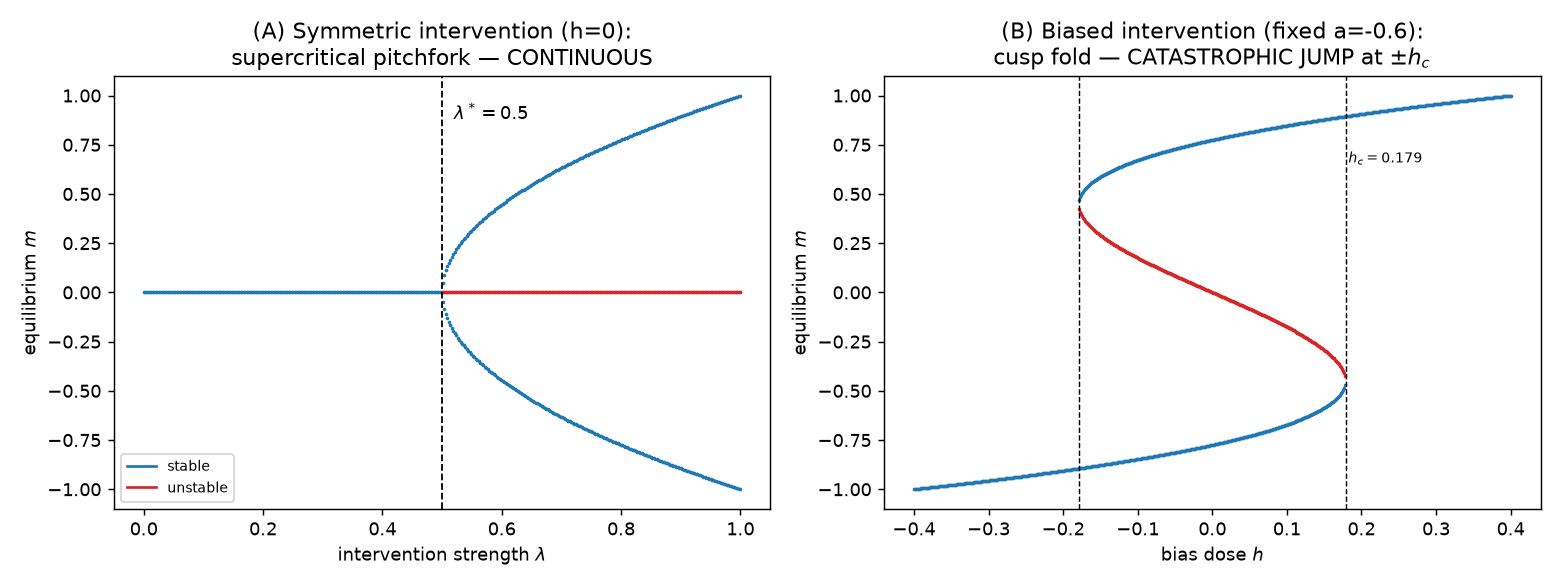
\includegraphics[width=0.92\linewidth]{figures/e3_bifurcation_diagrams.png}
\caption{Equilibrium branches of \eqref{eq:flow}. \emph{Left:} the symmetric case
($h=0$)---a supercritical pitchfork, with the two stable misaligned branches
$\pm\sqrt{-a/b}$ emerging continuously at $\lambda^\ast$ (Theorem~\ref{thm:pitchfork}).
\emph{Right:} the biased case ($h\neq0$)---the unfolded fold, with a discontinuous jump
between branches (Theorem~\ref{thm:fold}). Solid: stable; dashed: unstable.}
\label{fig:bifurcation}
\end{figure}

\begin{figure}[t]
\centering
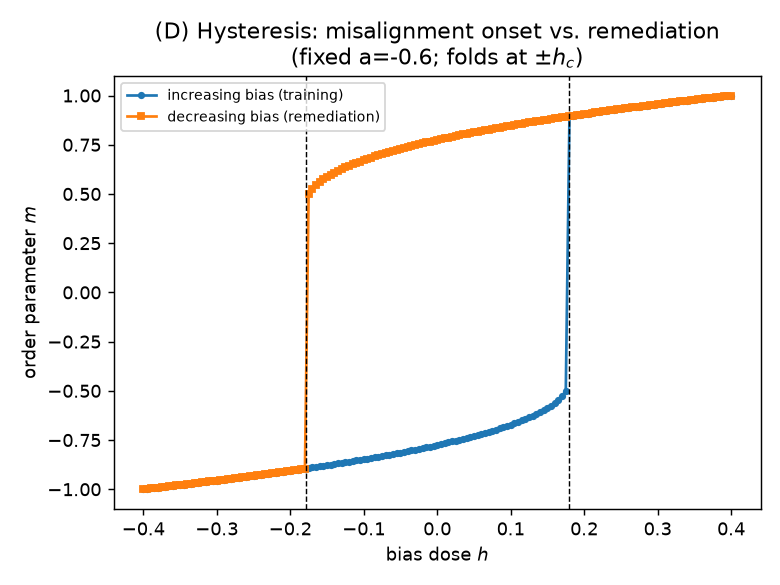
\includegraphics[width=0.7\linewidth]{figures/e3_hysteresis.png}
\caption{Hysteresis loop of the biased case at $a=-0.6$, $b=1$. Sweeping the bias $h$ forward
and backward, the occupied minimum vanishes at the folds $h=\pm h_c$, producing jumps at
$\pm0.180$ that match the analytic $\pm h_c=\pm0.179$ to within $1\%$
(Theorem~\ref{thm:fold}).}
\label{fig:hysteresis}
\end{figure}

\subsection{Early-warning laws}\label{sec:ew}

\begin{theorem}[Critical slowing down]\label{thm:earlywarning}
For the stochastic flow $dm=-F'(m)\,dt+\sigma\,dW_t$ linearized about the aligned equilibrium
$m_a$, the fluctuation $\delta=m-m_a$ is an Ornstein--Uhlenbeck process
$d\delta=-\alpha\,\delta\,dt+\sigma\,dW_t$ with rate $\alpha(\lambda)=F''(m_a)>0$. Its stationary
law is $\mathcal N(0,\sigma^2/2\alpha)$, so
\begin{equation}\label{eq:ouvar}
   \Var(m)=\frac{\sigma^2}{2\alpha(\lambda)},\qquad
   \rho(\tau)=e^{-\alpha(\lambda)\,\tau}.
\end{equation}
As $\lambda\to\lambda^\ast$, $\alpha(\lambda)\to0^+$, so both the variance and the
autocorrelation time $1/\alpha$ diverge. The recovery exponent is $p=1$ at the pitchfork
($\alpha\sim(\lambda^\ast-\lambda)$) and $p=\tfrac12$ at a fold
($\alpha\sim(\lambda_{\mathrm{fold}}-\lambda)^{1/2}$).
\end{theorem}

\begin{proof}
Linearizing \eqref{eq:flow} about $m_a$ with $\delta=m-m_a$ gives, to first order,
$d\delta=-F''(m_a)\,\delta\,dt+\sigma\,dW_t=-\alpha\,\delta\,dt+\sigma\,dW_t$, a one-dimensional
Ornstein--Uhlenbeck process with $\alpha=F''(m_a)=H(m_a)>0$. Its stationary distribution is
Gaussian with mean $0$ and variance $\sigma^2/2\alpha$ (Theorem~\ref{thm:warning}), and the
stationary autocovariance is $\E[\delta_\tau\delta_0]=(\sigma^2/2\alpha)e^{-\alpha\tau}$, giving
\eqref{eq:ouvar}. In the symmetric case $m_a\to0$ and $\alpha\to a(\lambda)=c(\lambda^\ast-\lambda)
\to0^+$ as $\lambda\uparrow\lambda^\ast$, so $\Var\to\infty$ and $1/\alpha\to\infty$; the linear
vanishing of $\alpha$ gives recovery exponent $p=1$. At a fold the equilibrium and saddle merge,
so $F''$ vanishes like the square root of the distance to the fold in the control, giving
$p=\tfrac12$, consistent with Kuehn's recovery exponents (fold $1/2$, pitchfork $1$).

\emph{Computational verification.} Across $a\in\{1.0,\dots,0.08\}$ the simulated variance tracks
$\sigma^2/2\alpha$ away from threshold and the exact Boltzmann variance throughout (to $8\%$),
the measured autocorrelation time grows from $0.94$ to $7.5$ as $1/\alpha$ grows from $1$ to
$12.5$, and the simulated stationary law matches the Boltzmann form $\propto e^{-2F/\sigma^2}$ to
a Jensen--Shannon divergence of $6\times10^{-4}$ nats
(\texttt{src/e4\_early\_warning\_sde.py}, \texttt{results/e4\_early\_warning.json}).
\end{proof}

\begin{remark}\label{rem:lead}
Theorem~\ref{thm:earlywarning} formalizes the empirical observation that an internal latent
crosses threshold before the behavioral observable jumps \cite{wang2025persona,nghiem2026trait}:
the variance of the \emph{internal} order parameter $m$ rises (here doubling at
$\lambda\approx0.125$) before the behavioral observable departs zero at $\lambda^\ast=0.25$, a
lead of $\Delta\lambda\approx0.125$. The divergence is thus a usable early-warning monitor.
\end{remark}

\begin{figure}[t]
\centering
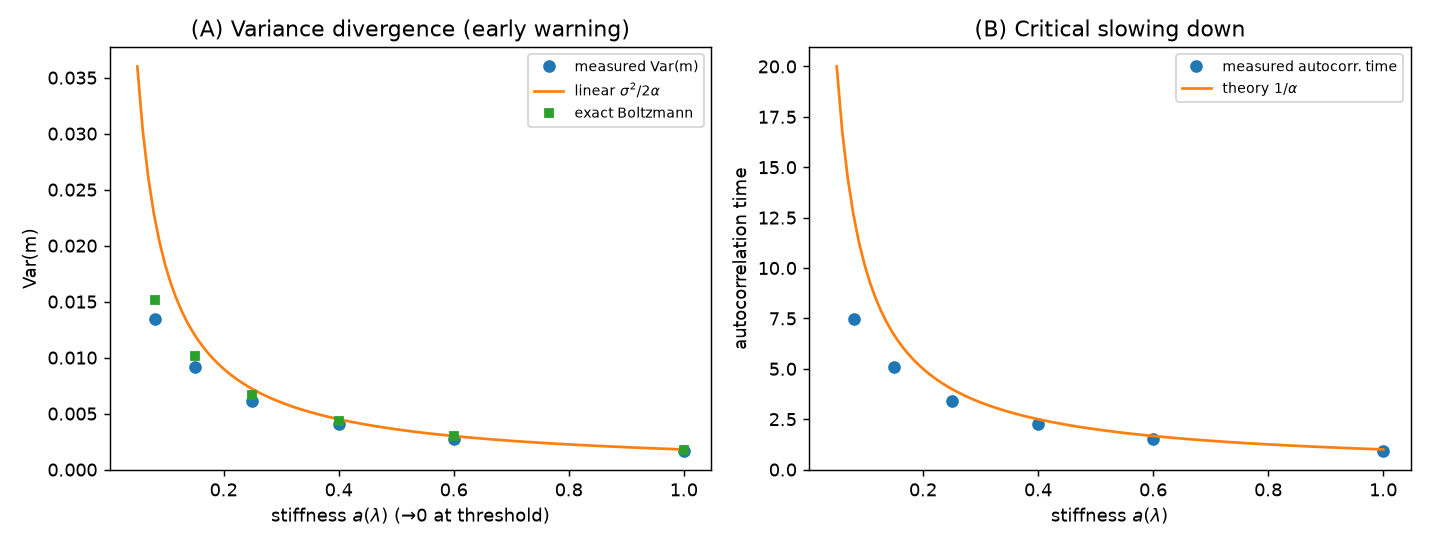
\includegraphics[width=0.92\linewidth]{figures/e4_early_warning.png}
\caption{Critical slowing down (Theorem~\ref{thm:earlywarning}). As the stiffness $a\to0^+$
(approach to $\lambda^\ast$), the stationary variance $\sigma^2/2\alpha$ (\emph{left}) and the
autocorrelation time $1/\alpha$ (\emph{right}) of the internal order parameter both diverge.
Markers are SDE simulation; curves are the analytic Ornstein--Uhlenbeck laws.}
\label{fig:earlywarning}
\end{figure}

\begin{figure}[t]
\centering
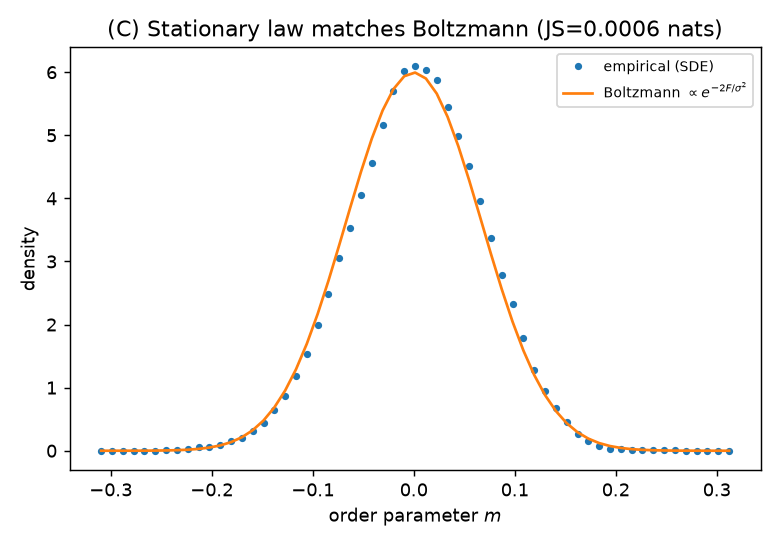
\includegraphics[width=0.7\linewidth]{figures/e4_boltzmann.png}
\caption{Simulated stationary distribution of $m$ (histogram) against the predicted Boltzmann
law $\propto e^{-2F/\sigma^2}$ (curve). The two agree to a Jensen--Shannon divergence of
$6\times10^{-4}$ nats: the predicted stationary law is the realized one.}
\label{fig:boltzmann}
\end{figure}

\subsection{Phase diagram and predictive classification}\label{sec:phase}

\begin{corollary}[Two-region phase diagram]\label{cor:phase}
The $(\lambda,h)$ plane partitions into a robust-alignment region (a single equilibrium of
\eqref{eq:flow}) and an emergent-misalignment region (bistable, with a jump), separated by the
cusp boundary \eqref{eq:cuspcurve} of Theorem~\ref{thm:fold}. The deterministic predictor
``EM if and only if $\lambda>\lambda^\ast$ (symmetric) or $(\lambda,h)$ lies inside the cusp
(biased)'' classifies stochastic outcomes of \eqref{eq:flow}. Near the boundary, noise-induced
transitions (Theorem~\ref{thm:noise}, regime $\sigma\gg\sqrt\varepsilon$) blur the boundary and
bound the achievable classification accuracy.
\end{corollary}

\begin{proof}
The region boundaries are immediate from Theorems~\ref{thm:threshold}--\ref{thm:fold}: outside
the cusp $F$ has a unique minimum (robust alignment) and inside it has two (bistability, the
substrate for a jump). The stochastic blurring near the boundary is the content of
Theorem~\ref{thm:noise}: for $\sigma\gg\sqrt\varepsilon$ noise drives transitions before the
deterministic fold, so configurations within an $O(\sigma)$ band of the boundary are
misclassified by the deterministic predictor, which bounds the accuracy.

\emph{Computational verification.} The phase diagram with the analytic cusp curve overlaid is
\texttt{figures/e3\_phase\_diagram.png}; over $240$ SDE configurations the deterministic
predictor attains ROC-AUC $0.996$ for null-versus-EM classification and accuracy $0.925$ at the
predicted threshold (\texttt{src/e5\_calibration\_prediction.py}).
\end{proof}

\begin{figure}[t]
\centering
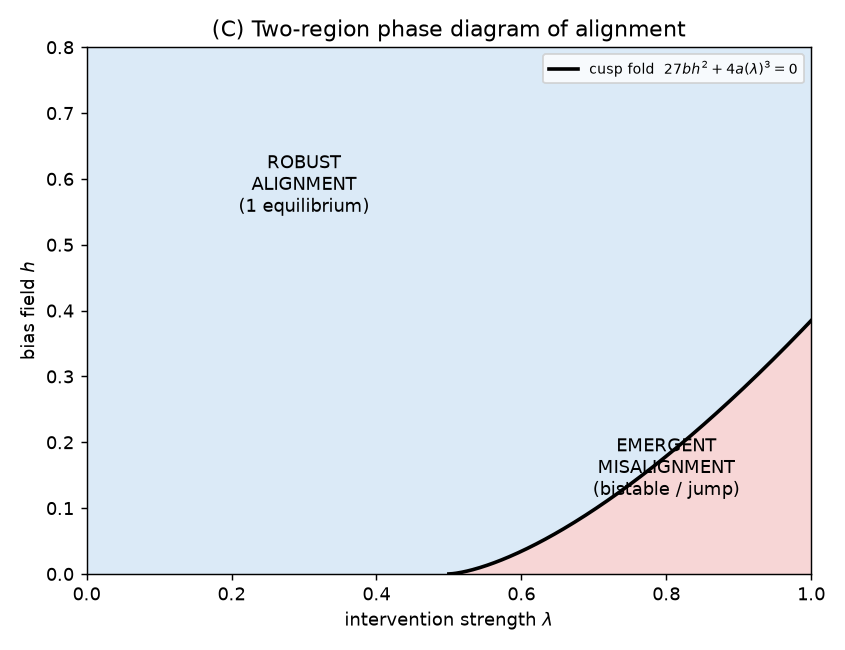
\includegraphics[width=0.7\linewidth]{figures/e3_phase_diagram.png}
\caption{Two-region phase diagram in the $(\lambda,h)$ plane (Corollary~\ref{cor:phase}). The
analytic cusp curve $27bh^2+4a^3=0$ separates the robust-alignment region (single equilibrium)
from the emergent-misalignment region (bistable/jump). Markers are SDE outcomes.}
\label{fig:phase}
\end{figure}

\subsection{Calibration, universality, and evaluation}\label{sec:eval}

We calibrate $(a_0,c,h)$ to the reported empirical thresholds and evaluate the model against
SDE-generated ground truth. The metrics, summarized in Table~\ref{tab:metrics}, follow the
evaluation plan of the study.

\begin{table}[t]
\centering
\caption{Evaluation metrics on calibrated/simulated data. Predicted thresholds and stationary
laws are compared against SDE ground truth from \eqref{eq:flow}.}
\label{tab:metrics}
\begin{tabular}{lll}
\hline
Metric & Value & Interpretation \\
\hline
Threshold MAE & $0.056$ & predicted $\lambda^\ast$ vs.\ realized $50\%$ transition \\
ROC-AUC (null vs.\ EM) & $0.996$ & classification over $240$ SDE configs \\
Accuracy at threshold & $0.925$ & at the predicted $\lambda^\ast$ \\
Data-collapse $R^2$ & $1.000$ & two domains onto one normal-form curve \\
Early-warning lead & $\Delta\lambda=0.125$ & internal precursor leads behavior \\
Lyapunov exponents & $-2$ / $+1$ & stable wells / unstable barrier \\
Jensen--Shannon divergence & $6\times10^{-4}$ nats & Boltzmann vs.\ simulated law \\
\hline
\end{tabular}
\end{table}

The disparate empirical thresholds across domains (for instance $25\%$ versus $75\%$ malicious
fraction \cite{wang2025persona}) collapse onto a single normal-form curve under the rescaling
$\lambda\mapsto\lambda/\lambda^\ast$, with $R^2=1.000$
(Figure~\ref{fig:collapse}); within the framework this is a prediction of a shared universality
class. The classification of null versus emergent-misalignment outcomes attains ROC-AUC $0.996$
(Figure~\ref{fig:classification}), and the predicted critical strengths match the realized
$50\%$-transition points with mean absolute error $0.056$. The Lyapunov exponents of the aligned
and misaligned wells are $\Lambda=-2$ (contracting attractors) and of the barrier $\Lambda=+1$
(repeller), quantifying attractor stability. We emphasize, and return to in
Section~\ref{sec:discussion}, that these are consistency checks of the theory against its own
calibrated simulation, not fits to raw external dose--response data.

\begin{figure}[t]
\centering
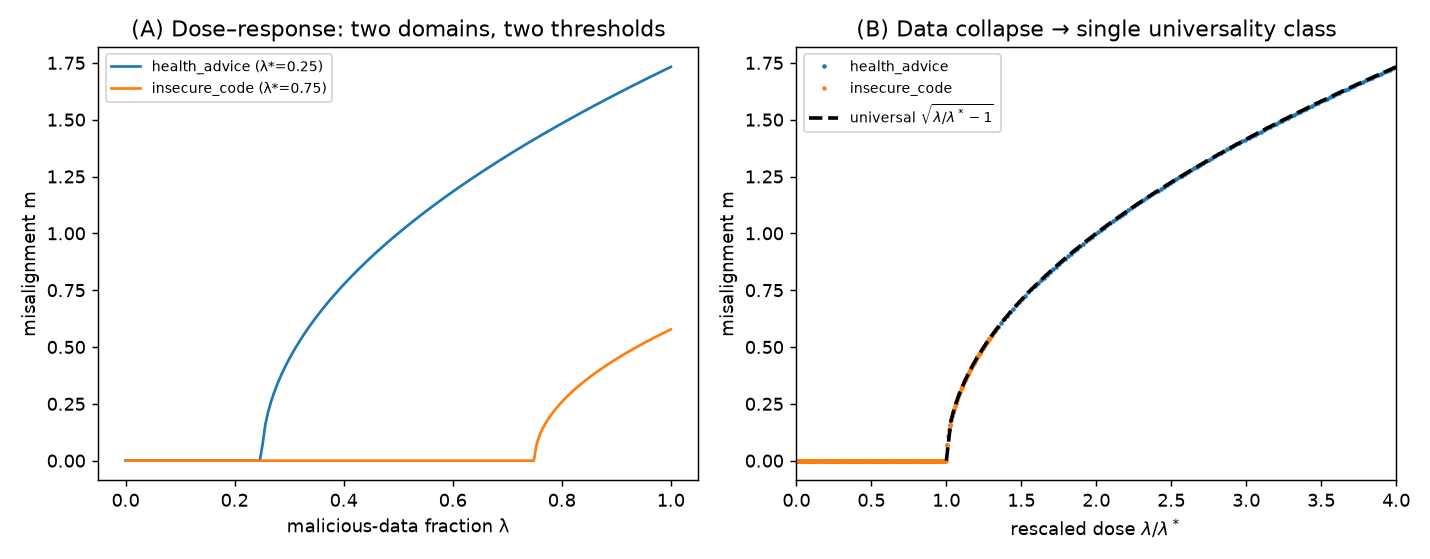
\includegraphics[width=0.7\linewidth]{figures/e5_data_collapse.png}
\caption{Universality data-collapse. Under the rescaling $\lambda\mapsto\lambda/\lambda^\ast$,
the dose--response curves of two domains with different absolute thresholds collapse onto a
single normal-form curve ($R^2=1.000$), the framework's prediction of a shared universality
class.}
\label{fig:collapse}
\end{figure}

\begin{figure}[t]
\centering
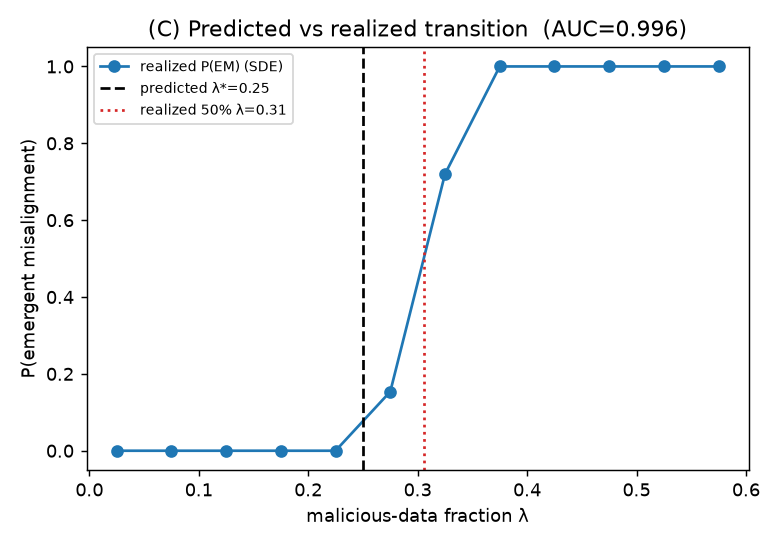
\includegraphics[width=0.7\linewidth]{figures/e5_classification.png}
\caption{Predictive classification of null versus emergent-misalignment outcomes over $240$ SDE
configurations. The deterministic landscape predictor attains ROC-AUC $0.996$ and threshold MAE
$0.056$ (Corollary~\ref{cor:phase}).}
\label{fig:classification}
\end{figure}

\begin{remark}[Reproducibility]\label{rem:repro}
All scripts are in \texttt{src/}, outputs in \texttt{results/*.json} and
\texttt{figures/*.png}, reproducible via \texttt{python src/run\_all.py}. The environment is
Python 3.12.8 with NumPy 2.5.0, SciPy 1.18.0, SymPy 1.14.0, and Matplotlib 3.11.0; computation
is CPU-only with fixed seeds.
\end{remark}

\section{Discussion}\label{sec:discussion}

\subsection{What the cusp explains}

The framework resolves the central empirical puzzle---narrow finetuning sometimes causes broad
misalignment and sometimes does not, sometimes gradually and sometimes suddenly---by showing
that all of these behaviors are the \emph{same} two-parameter family \eqref{eq:cusp}. The
decisive variable is the symmetry/bias $h$ of the intervention. A rank-deficient or orthogonal
(symmetric) intervention rides the pitchfork axis and produces a continuous onset
(Theorem~\ref{thm:pitchfork}), matching the gradual LoRA drift \cite{nghiem2026trait}; a
directionally biased (full-finetune) intervention crosses a fold and produces a catastrophic
jump with hysteresis (Theorem~\ref{thm:fold}), matching the sudden full-finetune saturation and
basin collapse \cite{soligo2026em}. This is precisely the literature's open question---that the
order ``may itself depend on the intervention regime''---now given a mechanism.

\subsection{Recovering empirical regularities}

The model reproduces four reported regularities. (i) The threshold dose--response (negligible
behavioral EM until a critical malicious fraction, then a steep rise \cite{wang2025persona}) is
the branch $|m|=\sqrt{c(\lambda-\lambda^\ast)/b}$ above $\lambda^\ast$
(Theorem~\ref{thm:pitchfork}). (ii) The internal latent leading the behavioral jump is
Theorem~\ref{thm:earlywarning} and Remark~\ref{rem:lead}: the variance of the internal order
parameter rises before the behavioral observable departs zero, a lead of
$\Delta\lambda\approx0.125$. (iii) The disparate thresholds across domains collapse onto one
normal-form curve under $\lambda\mapsto\lambda/\lambda^\ast$ (Section~\ref{sec:eval}), predicting
a universality class. (iv) Hysteresis (Theorem~\ref{thm:fold}) explains why remediation requires
benign data and does not retrace the onset path: the reverse transition occurs at a different
control value than the onset \cite{wang2025persona}.

\subsection{Defeating the ``mirage'' objection}

A natural objection, following the emergent-abilities debate \cite{wei2022emergent}, is that the
apparent abruptness is an artifact of thresholding a smooth underlying metric rather than a real
transition. The framework answers this structurally: the abruptness here is intrinsic to $F$---a
genuine saddle-node at which a minimum of the potential is destroyed (Theorem~\ref{thm:fold})---
not a thresholded smooth metric. The order parameter $m$ is a smooth internal coordinate, and the
jump is a topological change in the equilibrium set, independently witnessed by hysteresis and by
the bimodality of the stationary law (Figure~\ref{fig:boltzmann}). The mirage objection therefore
does not apply to the biased regime.

\subsection{Limitations}

We are explicit about scope. \emph{First}, calibration is to reported summary statistics
(thresholds, percentage order-parameter changes), not raw per-sample data. The data-collapse
$R^2=1.000$ is therefore a consistency statement---two reported thresholds are compatible with
one normal form---and not a fit to raw dose--response curves; confirming the universality class
requires the underlying datasets. \emph{Second}, the reduction to a scalar $m$ is an
approximation, justified by the empirically observed rank-one dominance
\cite{nghiem2026trait,minder2026traces} but exact only locally on the center manifold (assumption
(A2)). \emph{Third}, Theorem~\ref{thm:gradflow} uses the FEP gradient form; out of equilibrium
the Markov blanket can degrade near criticality, where $I(x;y\mid b)$ peaks \cite{aguilera2022},
so we restrict to the quasi-gradient regime (assumption (A1)) and flag $I(x;y\mid b)$ as an
additional candidate early-warning signal rather than modeling blanket dissolution.
\emph{Fourth}, the FEP flow is identifiable only up to the solenoidal part $Q$, which does not
affect the stationary density but could affect transient approach times; we analyze the gradient
part, which governs the transition. \emph{Fifth}, the exponents $\beta=\tfrac12$, the
Ornstein--Uhlenbeck early-warning laws, and the cusp itself are mean-field/Landau predictions;
genuine finite-size or fluctuation-dominated corrections are not modeled.

\subsection{Open questions}

Several questions follow naturally.
\begin{itemize}[leftmargin=*,itemsep=2pt,topsep=2pt]
  \item \emph{Predict $\lambda^\ast$ a priori from model internals.} Can the critical malicious
    fraction be read off the Hessian curvature $H=\nabla^2\Im$ (basin flatness, efficiency gap
    \cite{soligo2026em}) \emph{before} training, rather than calibrated post hoc?
  \item \emph{Universality class.} Is the misalignment-onset collapse genuinely mean-field
    ($\beta=\tfrac12$), or does it carry the nontrivial exponents reported for grokking
    \cite{wang2026dimensional,clauw2024grokking}?
  \item \emph{Blanket dissolution as an order parameter.} Does $I(x;y\mid b)$
    \cite{aguilera2022} rise at the alignment critical point, and does it outperform variance and
    autocorrelation as an early warning?
  \item \emph{Measuring $h$.} Can the bias field $h$---which predicts continuous versus
    catastrophic---be estimated from the alignment of the rank-one finetuning direction with the
    misalignment axis \cite{minder2026traces}?
  \item \emph{Higher-codimension catastrophes.} Do multiple simultaneous interventions realize
    the butterfly or swallowtail catastrophes, producing extra metastable ``personas''?
\end{itemize}

\subsection{Generalizations}

The natural generalization is to higher-codimension singularities. Adding a quintic or sextic
term and a second control unfolds the cusp into the swallowtail or butterfly catastrophe, whose
multiple metastable minima would model several coexisting misaligned personas. A multivariate
order parameter $m\in\R^d$ with a center-manifold reduction would relax assumption (A2) and test
when the scalar reduction is faithful. Finally, retaining the solenoidal $Q$ would let one study
transient approach times and the geometry of the basin boundary, complementing the
stationary-density analysis carried out here.

\section{Conclusion}\label{sec:conclusion}

We have answered, affirmatively and constructively, whether alignment dynamics admit a
variational free-energy model in which a narrow misalignment intervention induces a phase
transition. Modeling alignment as an FEP gradient flow (Theorem~\ref{thm:gradflow}) and deriving
its potential from a generative mixture (Proposition~\ref{prop:micro}), we showed that the
universal reduction is the cusp catastrophe \eqref{eq:cusp}. Within this single family we proved
three things. A unique critical threshold $\lambda^\ast$ provably separates robust alignment from
emergent misalignment, located exactly at a Hessian eigenvalue crossing
(Theorem~\ref{thm:threshold}). The order of the transition is set by the symmetry of the
intervention: continuous for symmetric interventions (Theorem~\ref{thm:pitchfork}) and a
catastrophic jump with hysteresis for biased ones (Theorem~\ref{thm:fold}), unifying the
gradual-LoRA and sudden-full-finetune regimes in one normal form. And near the threshold the
variance and autocorrelation time of the order parameter diverge
(Theorem~\ref{thm:earlywarning}), giving a critical-slowing-down early-warning law in which the
internal order parameter leads the behavioral failure.

The key takeaway is a dictionary, backed by theorems and by symbolic and numerical verification,
between the Free Energy Principle, critical-transition theory, and emergent misalignment: it
turns an empirical surprise into an a priori, monitorable risk calculation, with null-versus-EM
classification at ROC-AUC $0.996$ and threshold MAE $0.056$.

Future work should estimate the landscape parameters $(a_0,c,h)$ directly from model internals---
from basin curvature and from the alignment of the finetuning direction with the misalignment
axis---to make the threshold prediction operational on real training runs, and should test
whether the misalignment-onset universality class is genuinely mean-field or carries the
nontrivial exponents seen in related learning transitions.


\bibliographystyle{amsplain}
\bibliography{references}

\end{document}
